\documentclass[11pt]{article}
\usepackage[textwidth=18.0cm, textheight=23.0cm, top=2.0cm]{geometry}
\usepackage{pst-all}
\usepackage{amssymb}
\usepackage{tikz}
\usepackage{underscore}\begin{document}
\pagestyle{empty}


ClassName: \underline{\textbf{Class_03.2bp-23}}
\par
BinSize: \underline{\textbf{40 × 40}}
\par
ReduceSize: \underline{\textbf{40 × 40}}
\par
TypeNum: \underline{\textbf{58}}
\par
Num: \underline{\textbf{60}}
\par
OutS: \underline{\textbf{24000}}
\par
InS: \underline{\textbf{19663}}
\par
Rate: \underline{\textbf{0.819}}
\par
UB: \underline{\textbf{15}}
\par
LB0: \underline{\textbf{15}}
\par
LB: \underline{\textbf{15}}
\par
LBWithCut: \underline{\textbf{15}}
\par
NodeCut: \underline{\textbf{0}}
\par
ExtendedNodeCnt: \underline{\textbf{1}}
\par
GenNodeCnt: \underline{\textbf{1}}
\par
PrimalNode: \underline{\textbf{0}}
\par
ColumnCount: \underline{\textbf{15}}
\par
TotalCutCount: \underline{\textbf{0}}
\par
RootCutCount: \underline{\textbf{0}}
\par
LPSolverCnt: \underline{\textbf{1}}
\par
PricingSolverCnt: \underline{\textbf{0}}
\par
BranchAndBoundNum: \underline{\textbf{1}}
\par
isOpt: \underline{\textbf{true}}
\par
TimeOnPrimal: \underline{\textbf{0.000 s}}
\par
TimeOnPricing: \underline{\textbf{0.000 s}}
\par
TimeOnRmp: \underline{\textbf{0.078 s}}
\par
TotalTime: \underline{\textbf{0.141 s}}
\par
\newpage


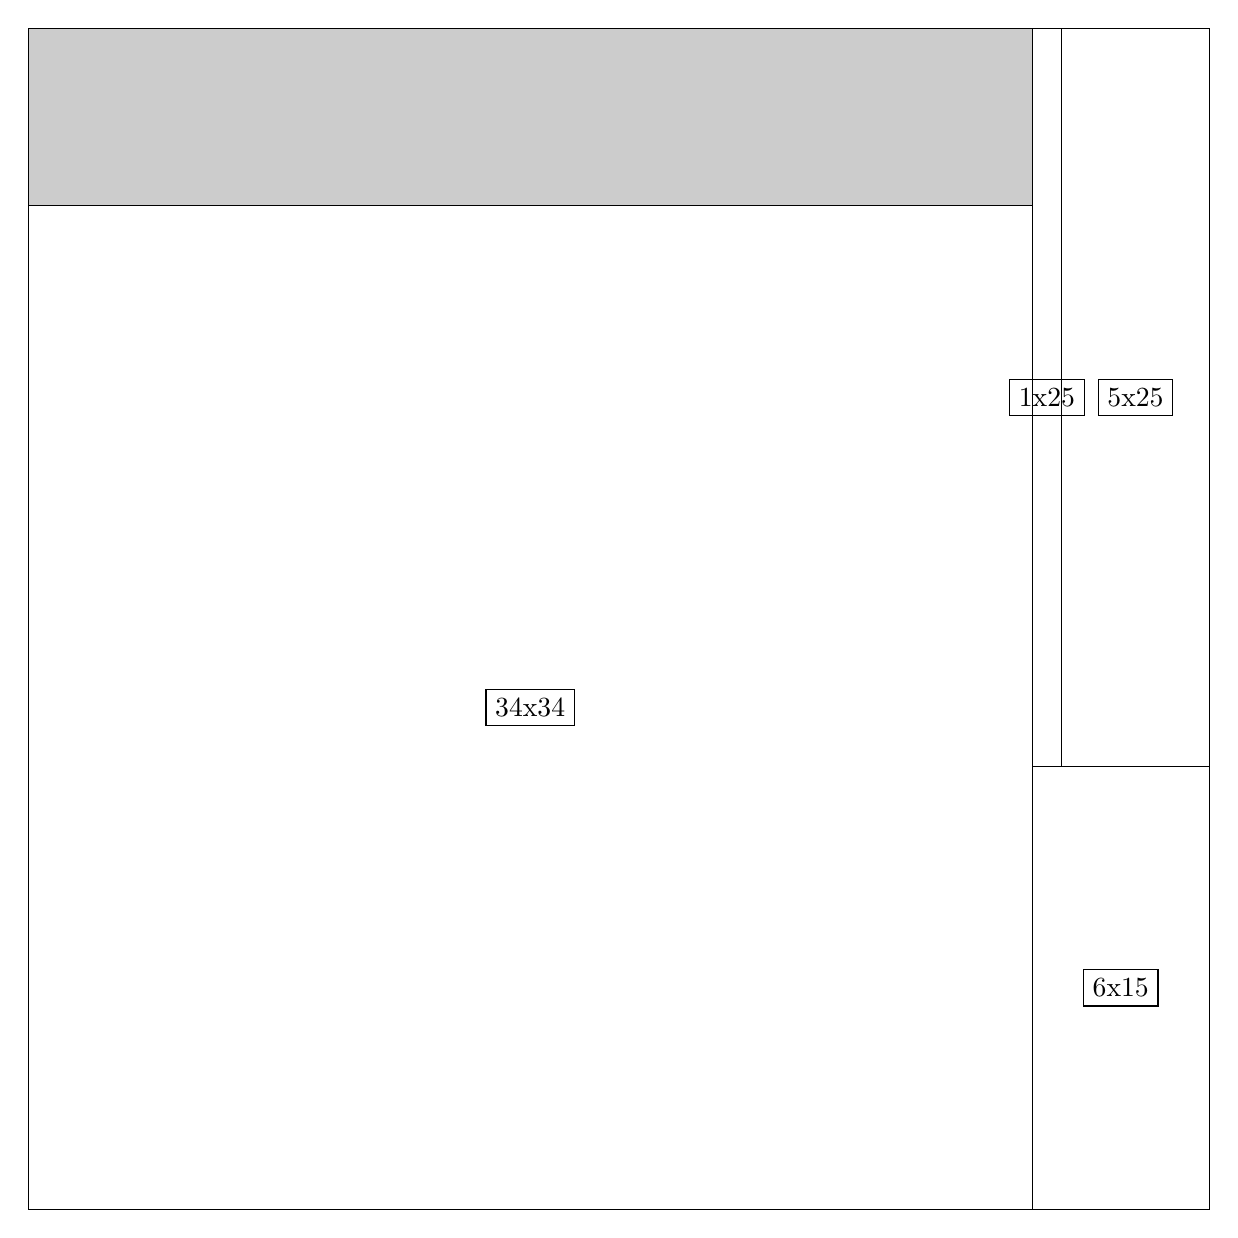
\begin{tikzpicture}[shorten >=1pt,scale=1.0,every node/.style={scale=1.0},->]
\tikzstyle{vertex}=[circle,fill=black!25,minimum size=14pt,inner sep=0pt]
\filldraw[fill=gray!40!white, draw=black] (0,0) rectangle (15.0,15.0);
\foreach \name/\x/\y/\w/\h in {34x34/0.0/0.0/12.75/12.75,5x25/13.125/5.625/1.875/9.375,6x15/12.75/0.0/2.25/5.625,1x25/12.75/5.625/0.375/9.375}
\filldraw[fill=white!40!white, draw=black] (\x,\y) rectangle node[draw] (\name) {\name} ++(\w,\h);
\end{tikzpicture}


w =34 , h =34 , x =0 , y =0 , v =1156
\par
w =5 , h =25 , x =35 , y =15 , v =125
\par
w =6 , h =15 , x =34 , y =0 , v =90
\par
w =1 , h =25 , x =34 , y =15 , v =25
\par
\newpage


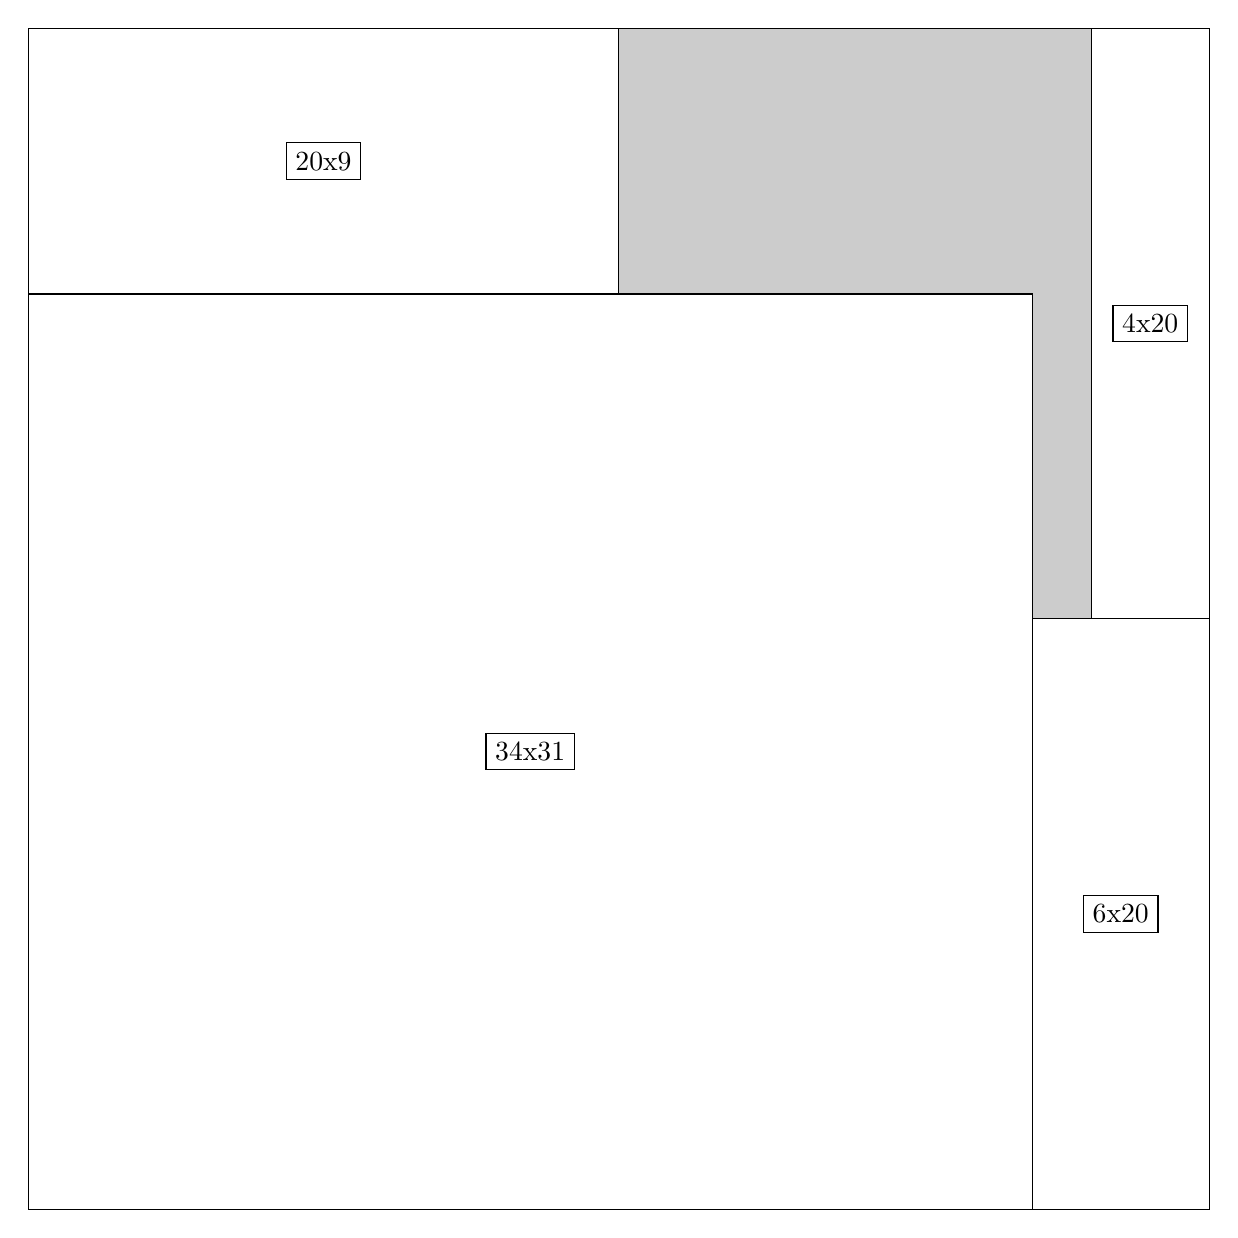
\begin{tikzpicture}[shorten >=1pt,scale=1.0,every node/.style={scale=1.0},->]
\tikzstyle{vertex}=[circle,fill=black!25,minimum size=14pt,inner sep=0pt]
\filldraw[fill=gray!40!white, draw=black] (0,0) rectangle (15.0,15.0);
\foreach \name/\x/\y/\w/\h in {34x31/0.0/0.0/12.75/11.625,20x9/0.0/11.625/7.5/3.375,6x20/12.75/0.0/2.25/7.5,4x20/13.5/7.5/1.5/7.5}
\filldraw[fill=white!40!white, draw=black] (\x,\y) rectangle node[draw] (\name) {\name} ++(\w,\h);
\end{tikzpicture}


w =34 , h =31 , x =0 , y =0 , v =1054
\par
w =20 , h =9 , x =0 , y =31 , v =180
\par
w =6 , h =20 , x =34 , y =0 , v =120
\par
w =4 , h =20 , x =36 , y =20 , v =80
\par
\newpage


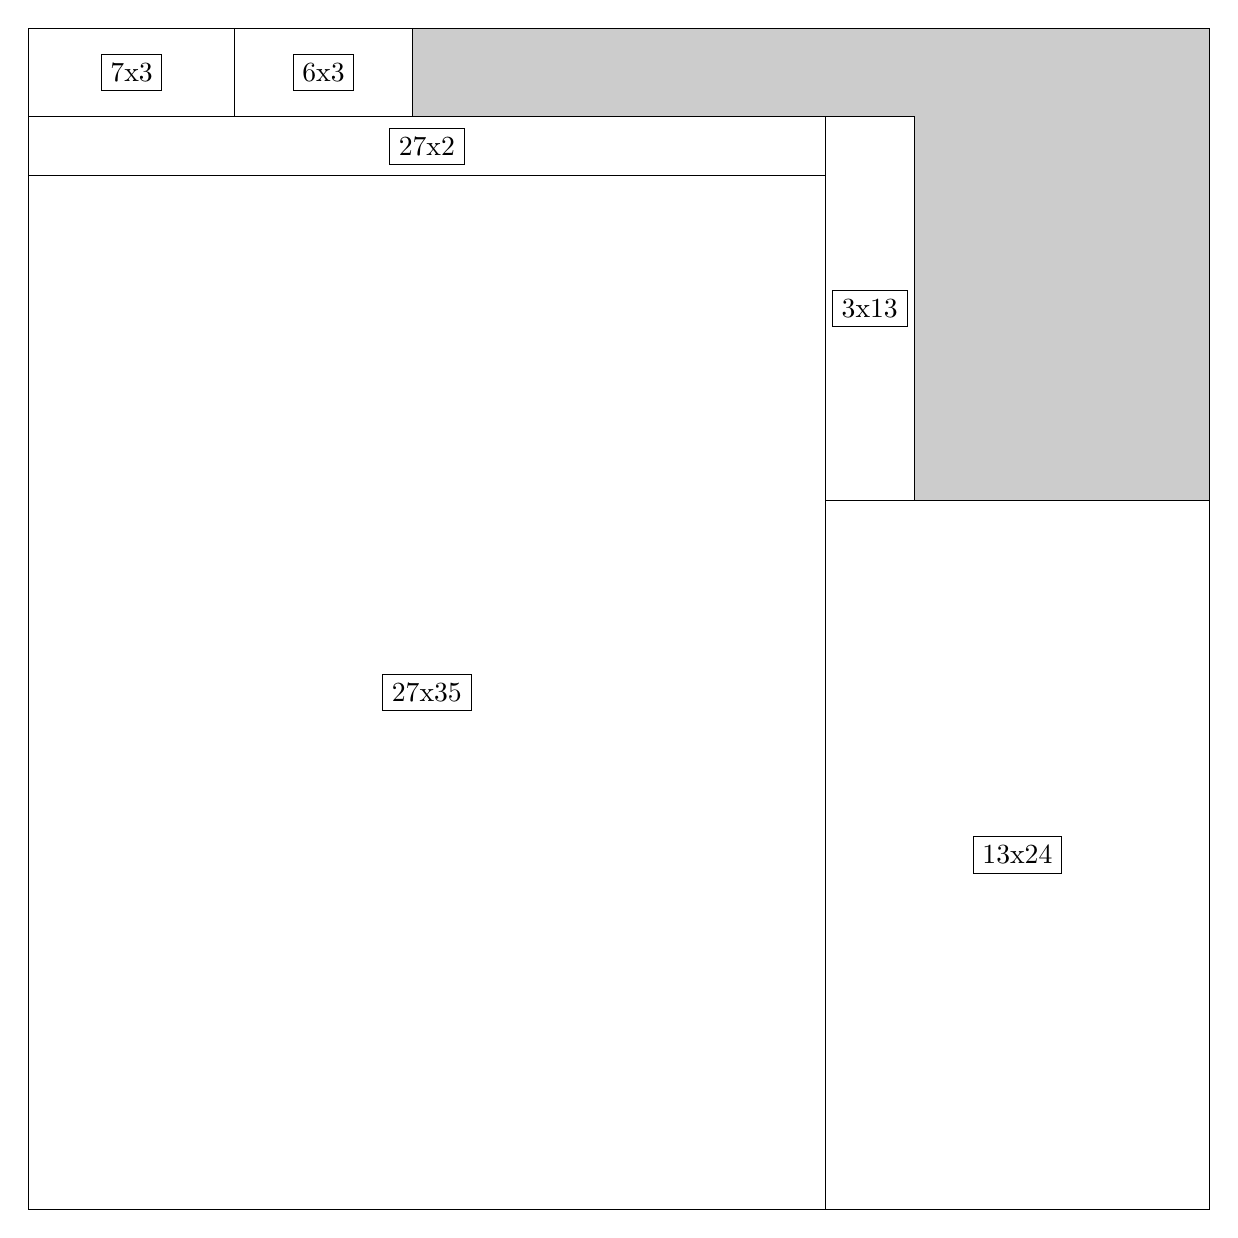
\begin{tikzpicture}[shorten >=1pt,scale=1.0,every node/.style={scale=1.0},->]
\tikzstyle{vertex}=[circle,fill=black!25,minimum size=14pt,inner sep=0pt]
\filldraw[fill=gray!40!white, draw=black] (0,0) rectangle (15.0,15.0);
\foreach \name/\x/\y/\w/\h in {27x35/0.0/0.0/10.125/13.125,13x24/10.125/0.0/4.875/9.0,27x2/0.0/13.125/10.125/0.75,3x13/10.125/9.0/1.125/4.875,7x3/0.0/13.875/2.625/1.125,6x3/2.625/13.875/2.25/1.125}
\filldraw[fill=white!40!white, draw=black] (\x,\y) rectangle node[draw] (\name) {\name} ++(\w,\h);
\end{tikzpicture}


w =27 , h =35 , x =0 , y =0 , v =945
\par
w =13 , h =24 , x =27 , y =0 , v =312
\par
w =27 , h =2 , x =0 , y =35 , v =54
\par
w =3 , h =13 , x =27 , y =24 , v =39
\par
w =7 , h =3 , x =0 , y =37 , v =21
\par
w =6 , h =3 , x =7 , y =37 , v =18
\par
\newpage


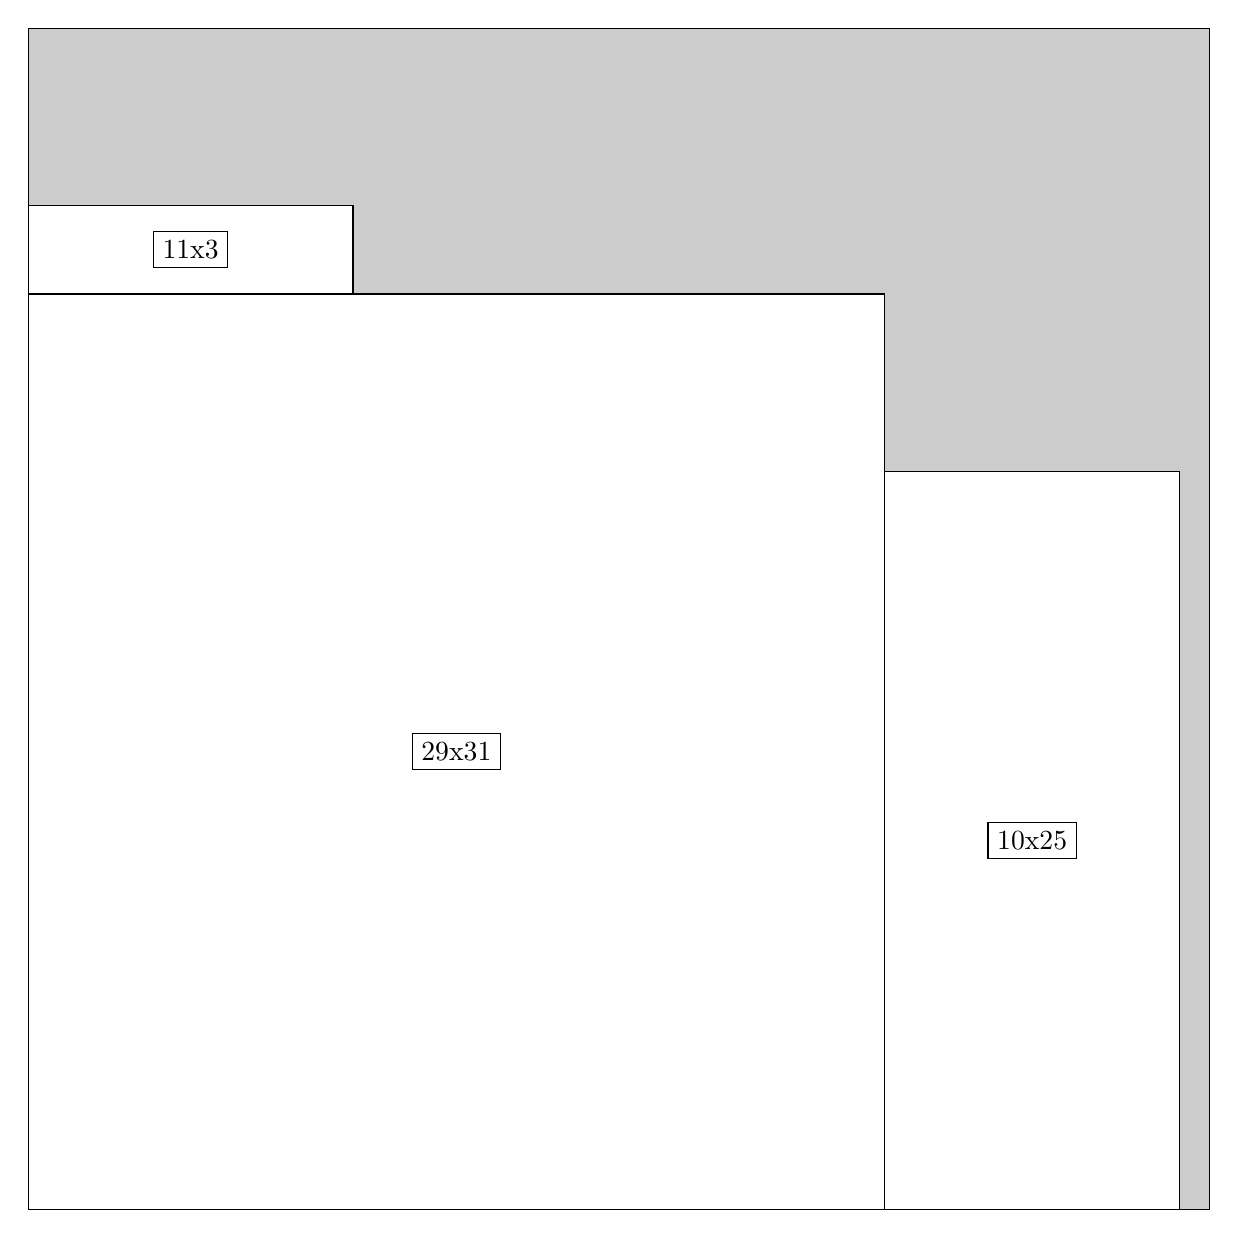
\begin{tikzpicture}[shorten >=1pt,scale=1.0,every node/.style={scale=1.0},->]
\tikzstyle{vertex}=[circle,fill=black!25,minimum size=14pt,inner sep=0pt]
\filldraw[fill=gray!40!white, draw=black] (0,0) rectangle (15.0,15.0);
\foreach \name/\x/\y/\w/\h in {29x31/0.0/0.0/10.875/11.625,10x25/10.875/0.0/3.75/9.375,11x3/0.0/11.625/4.125/1.125}
\filldraw[fill=white!40!white, draw=black] (\x,\y) rectangle node[draw] (\name) {\name} ++(\w,\h);
\end{tikzpicture}


w =29 , h =31 , x =0 , y =0 , v =899
\par
w =10 , h =25 , x =29 , y =0 , v =250
\par
w =11 , h =3 , x =0 , y =31 , v =33
\par
\newpage


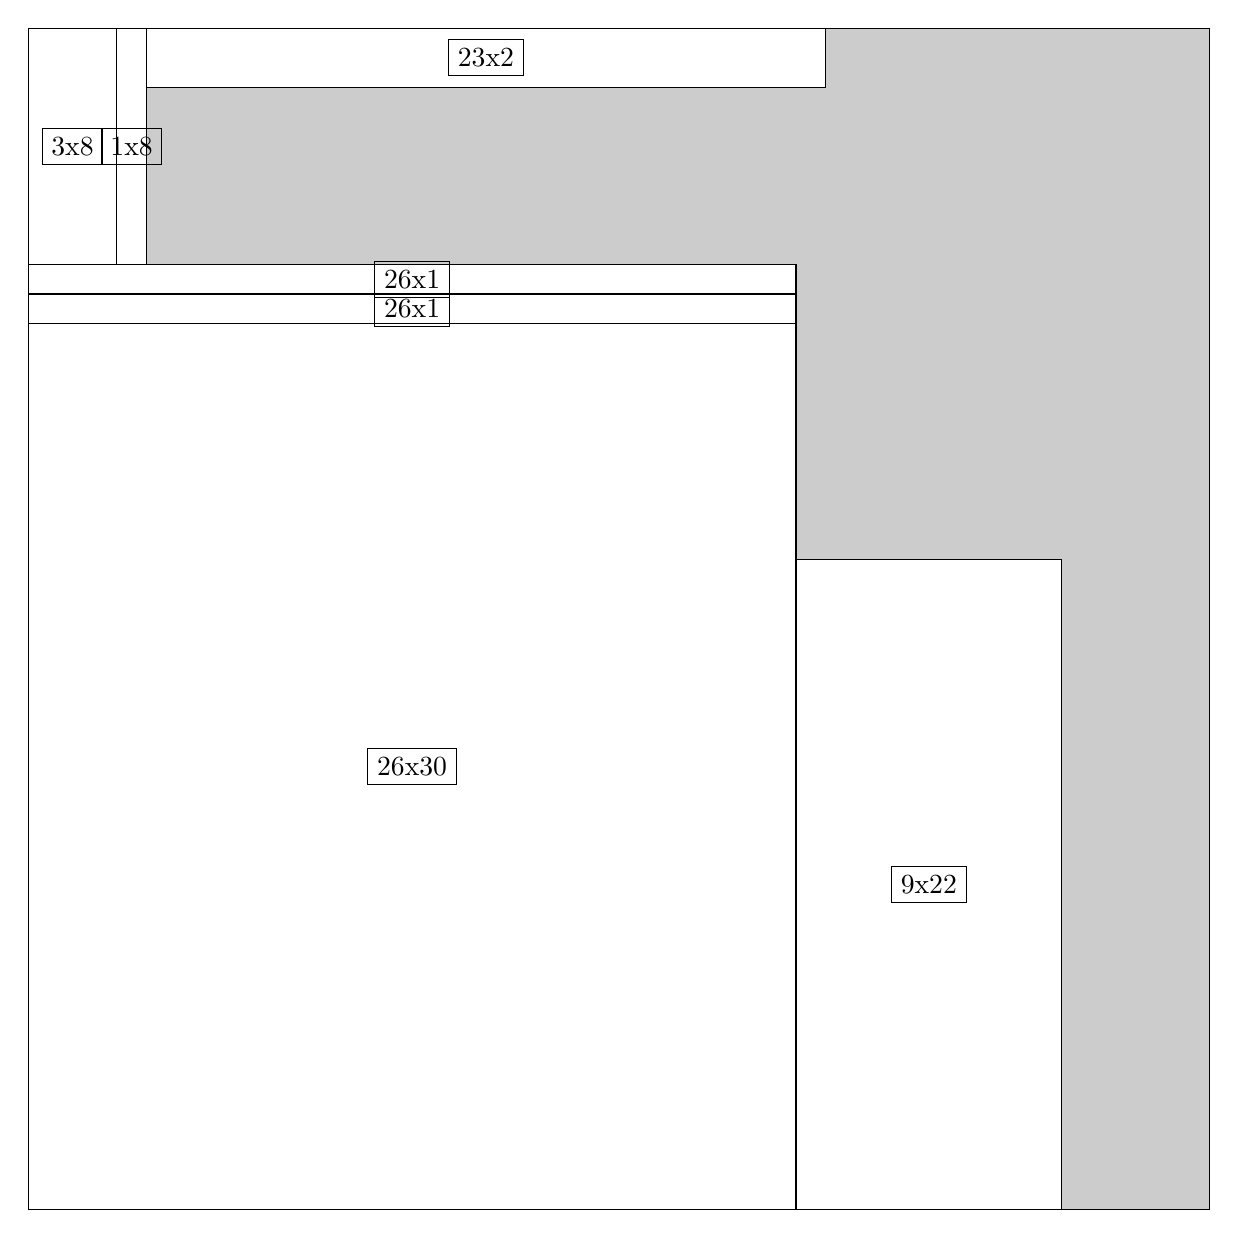
\begin{tikzpicture}[shorten >=1pt,scale=1.0,every node/.style={scale=1.0},->]
\tikzstyle{vertex}=[circle,fill=black!25,minimum size=14pt,inner sep=0pt]
\filldraw[fill=gray!40!white, draw=black] (0,0) rectangle (15.0,15.0);
\foreach \name/\x/\y/\w/\h in {26x30/0.0/0.0/9.75/11.25,9x22/9.75/0.0/3.375/8.25,23x2/1.5/14.25/8.625/0.75,26x1/0.0/11.25/9.75/0.375,26x1/0.0/11.625/9.75/0.375,3x8/0.0/12.0/1.125/3.0,1x8/1.125/12.0/0.375/3.0}
\filldraw[fill=white!40!white, draw=black] (\x,\y) rectangle node[draw] (\name) {\name} ++(\w,\h);
\end{tikzpicture}


w =26 , h =30 , x =0 , y =0 , v =780
\par
w =9 , h =22 , x =26 , y =0 , v =198
\par
w =23 , h =2 , x =4 , y =38 , v =46
\par
w =26 , h =1 , x =0 , y =30 , v =26
\par
w =26 , h =1 , x =0 , y =31 , v =26
\par
w =3 , h =8 , x =0 , y =32 , v =24
\par
w =1 , h =8 , x =3 , y =32 , v =8
\par
\newpage


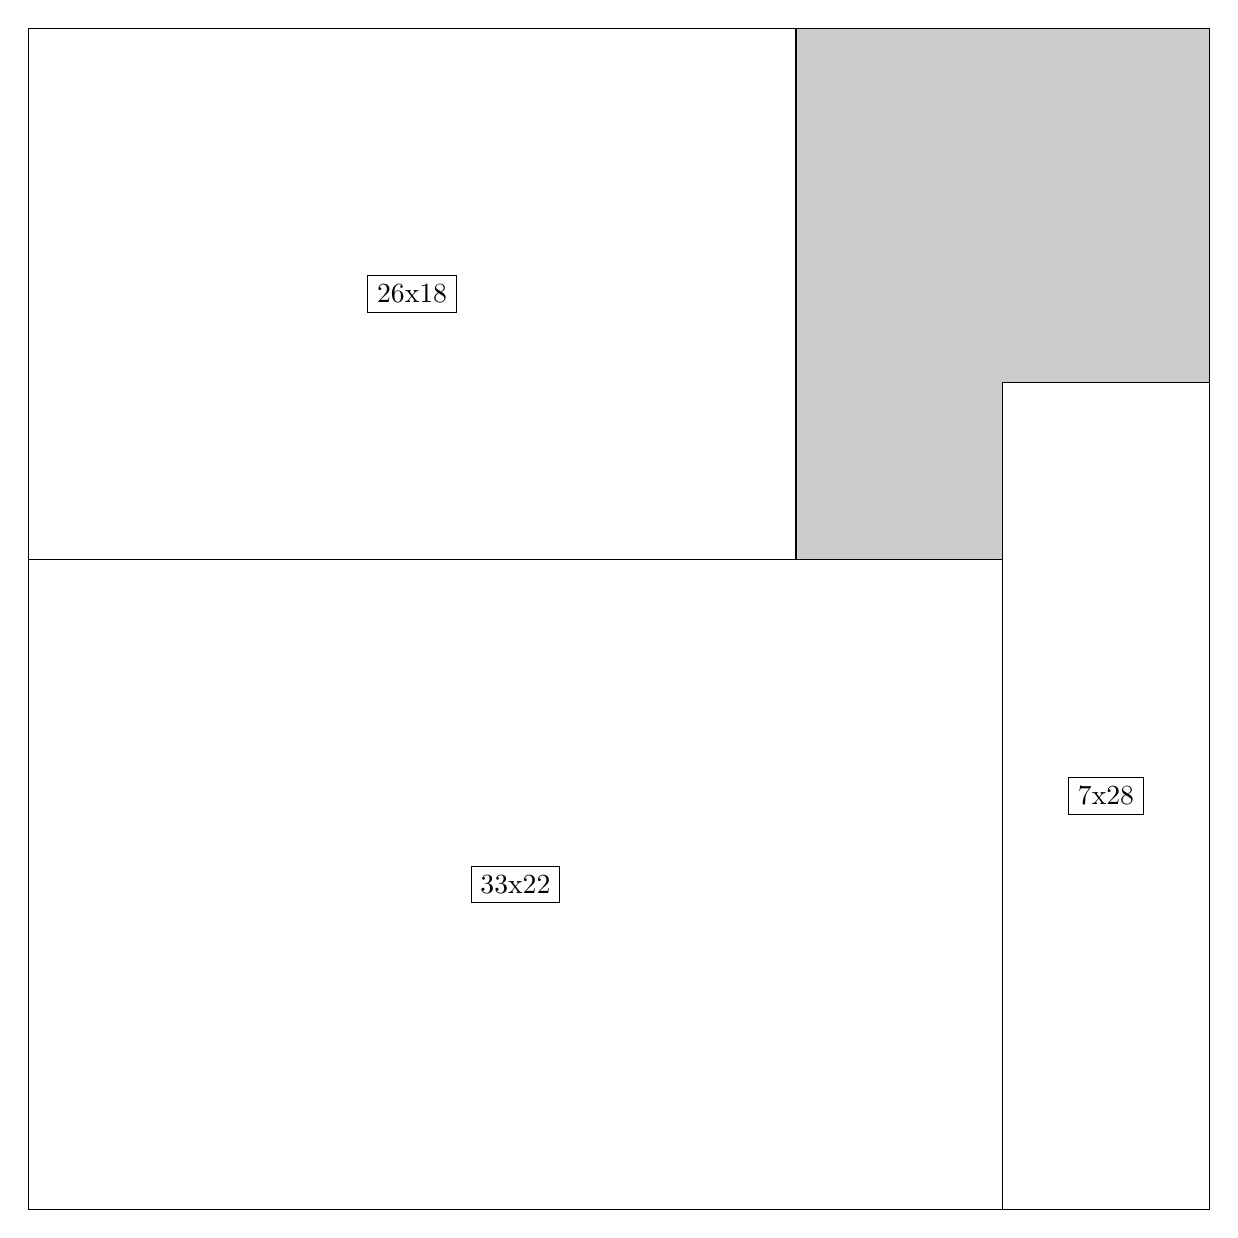
\begin{tikzpicture}[shorten >=1pt,scale=1.0,every node/.style={scale=1.0},->]
\tikzstyle{vertex}=[circle,fill=black!25,minimum size=14pt,inner sep=0pt]
\filldraw[fill=gray!40!white, draw=black] (0,0) rectangle (15.0,15.0);
\foreach \name/\x/\y/\w/\h in {33x22/0.0/0.0/12.375/8.25,26x18/0.0/8.25/9.75/6.75,7x28/12.375/0.0/2.625/10.5}
\filldraw[fill=white!40!white, draw=black] (\x,\y) rectangle node[draw] (\name) {\name} ++(\w,\h);
\end{tikzpicture}


w =33 , h =22 , x =0 , y =0 , v =726
\par
w =26 , h =18 , x =0 , y =22 , v =468
\par
w =7 , h =28 , x =33 , y =0 , v =196
\par
\newpage


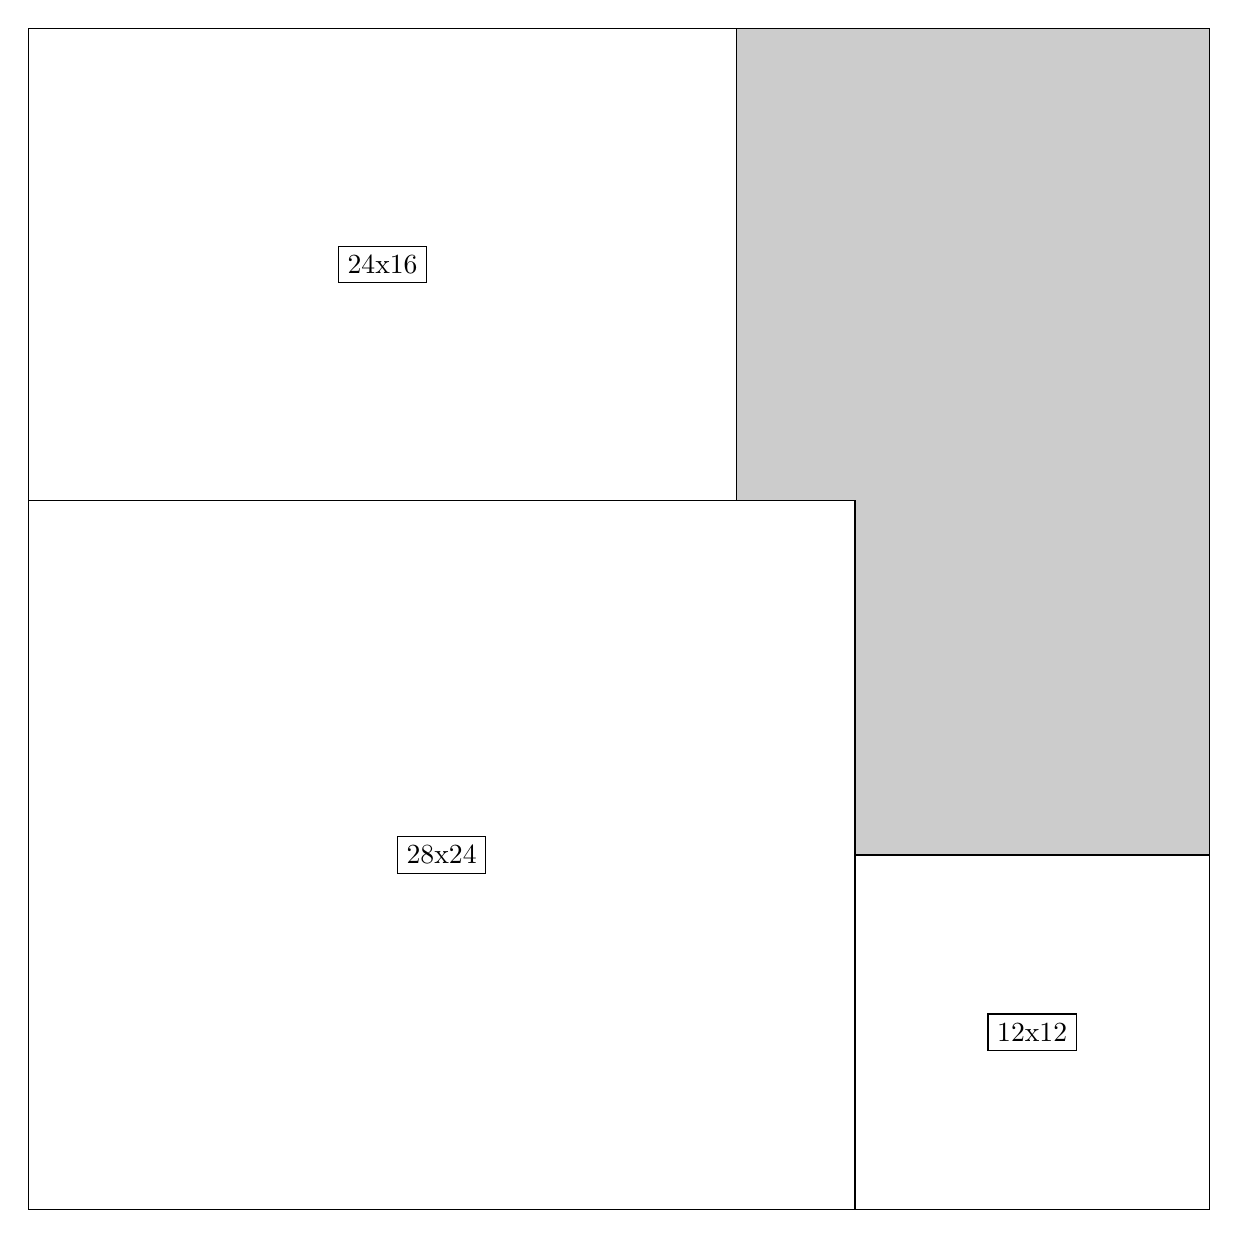
\begin{tikzpicture}[shorten >=1pt,scale=1.0,every node/.style={scale=1.0},->]
\tikzstyle{vertex}=[circle,fill=black!25,minimum size=14pt,inner sep=0pt]
\filldraw[fill=gray!40!white, draw=black] (0,0) rectangle (15.0,15.0);
\foreach \name/\x/\y/\w/\h in {12x12/10.5/0.0/4.5/4.5,28x24/0.0/0.0/10.5/9.0,24x16/0.0/9.0/9.0/6.0}
\filldraw[fill=white!40!white, draw=black] (\x,\y) rectangle node[draw] (\name) {\name} ++(\w,\h);
\end{tikzpicture}


w =12 , h =12 , x =28 , y =0 , v =144
\par
w =28 , h =24 , x =0 , y =0 , v =672
\par
w =24 , h =16 , x =0 , y =24 , v =384
\par
\newpage


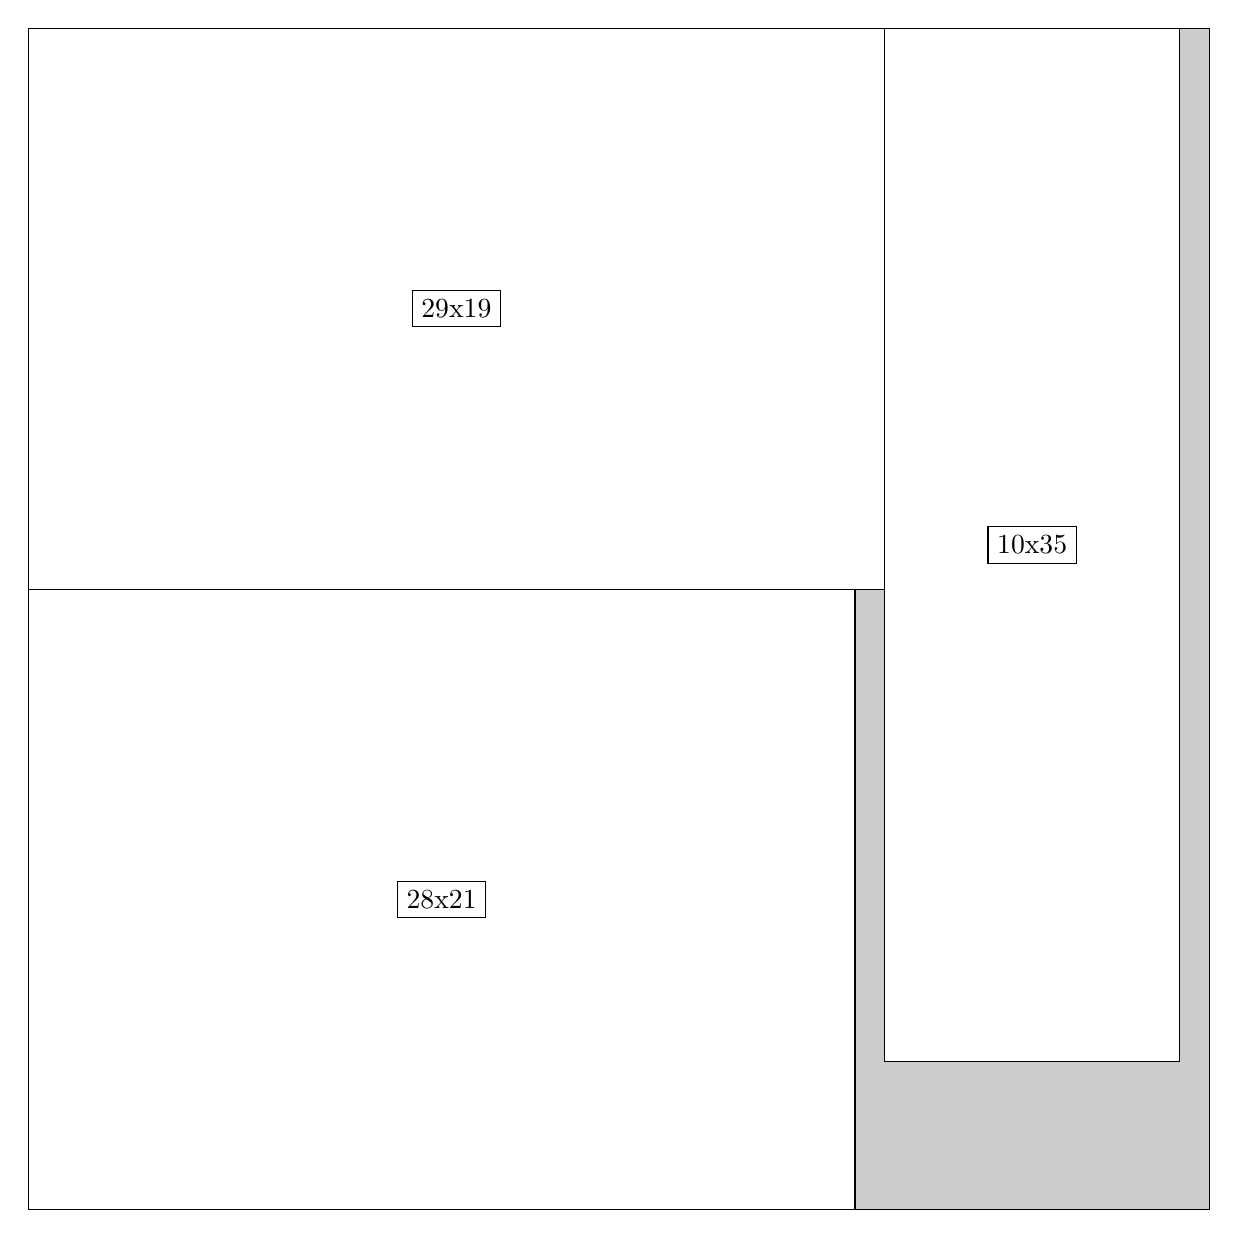
\begin{tikzpicture}[shorten >=1pt,scale=1.0,every node/.style={scale=1.0},->]
\tikzstyle{vertex}=[circle,fill=black!25,minimum size=14pt,inner sep=0pt]
\filldraw[fill=gray!40!white, draw=black] (0,0) rectangle (15.0,15.0);
\foreach \name/\x/\y/\w/\h in {28x21/0.0/0.0/10.5/7.875,29x19/0.0/7.875/10.875/7.125,10x35/10.875/1.875/3.75/13.125}
\filldraw[fill=white!40!white, draw=black] (\x,\y) rectangle node[draw] (\name) {\name} ++(\w,\h);
\end{tikzpicture}


w =28 , h =21 , x =0 , y =0 , v =588
\par
w =29 , h =19 , x =0 , y =21 , v =551
\par
w =10 , h =35 , x =29 , y =5 , v =350
\par
\newpage


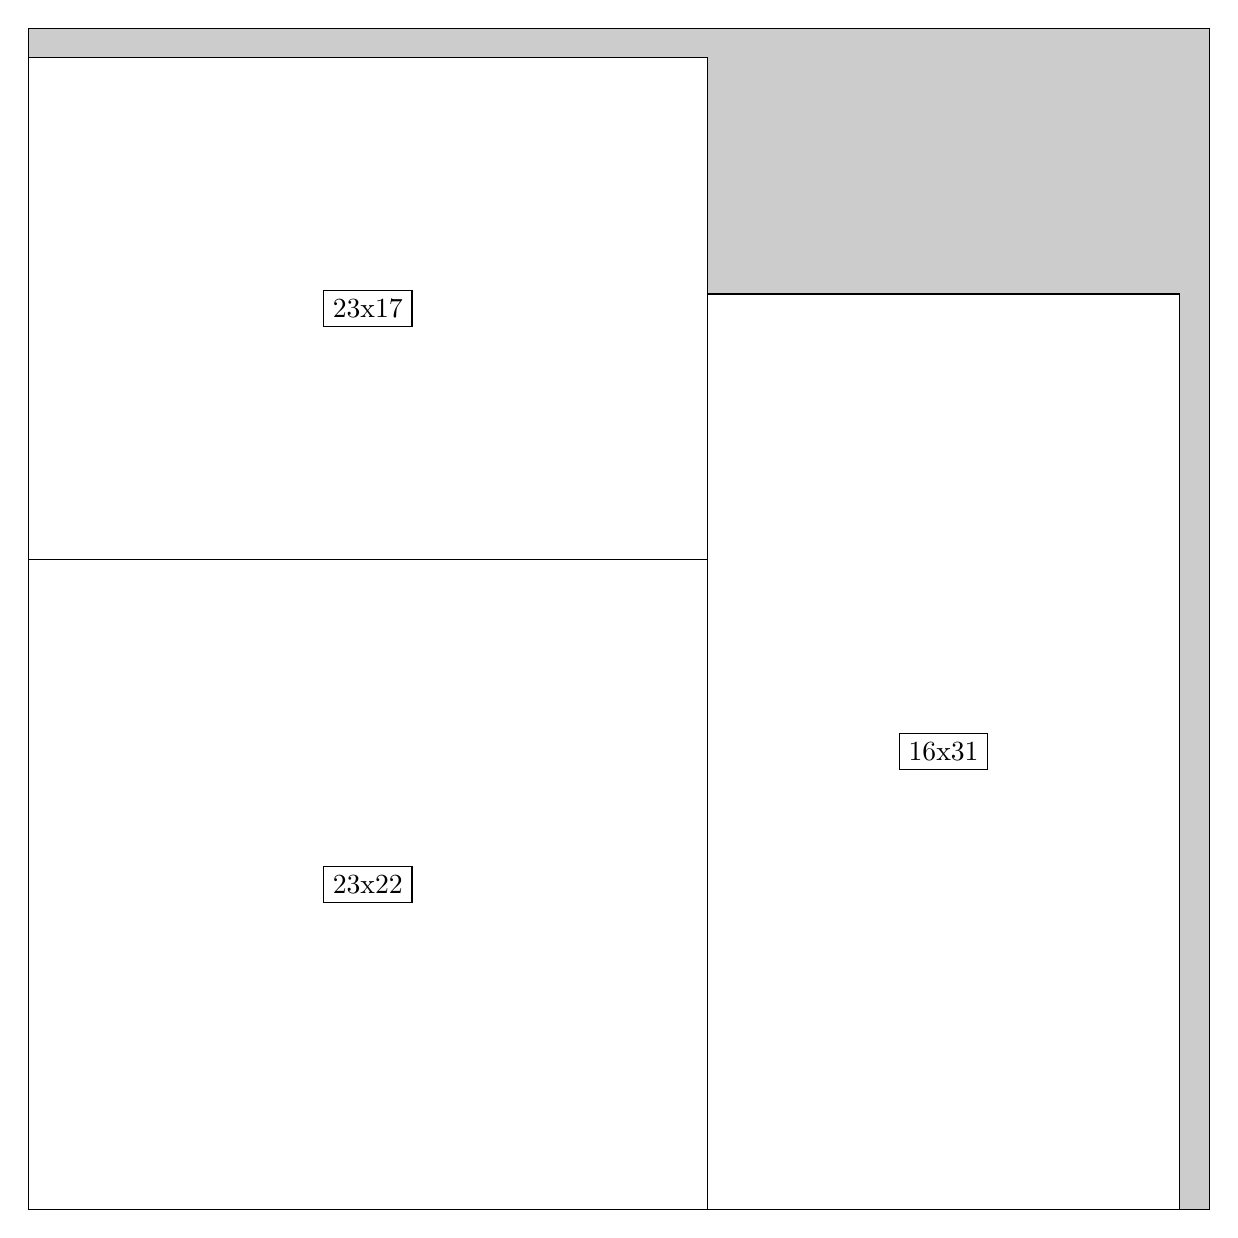
\begin{tikzpicture}[shorten >=1pt,scale=1.0,every node/.style={scale=1.0},->]
\tikzstyle{vertex}=[circle,fill=black!25,minimum size=14pt,inner sep=0pt]
\filldraw[fill=gray!40!white, draw=black] (0,0) rectangle (15.0,15.0);
\foreach \name/\x/\y/\w/\h in {23x22/0.0/0.0/8.625/8.25,16x31/8.625/0.0/6.0/11.625,23x17/0.0/8.25/8.625/6.375}
\filldraw[fill=white!40!white, draw=black] (\x,\y) rectangle node[draw] (\name) {\name} ++(\w,\h);
\end{tikzpicture}


w =23 , h =22 , x =0 , y =0 , v =506
\par
w =16 , h =31 , x =23 , y =0 , v =496
\par
w =23 , h =17 , x =0 , y =22 , v =391
\par
\newpage


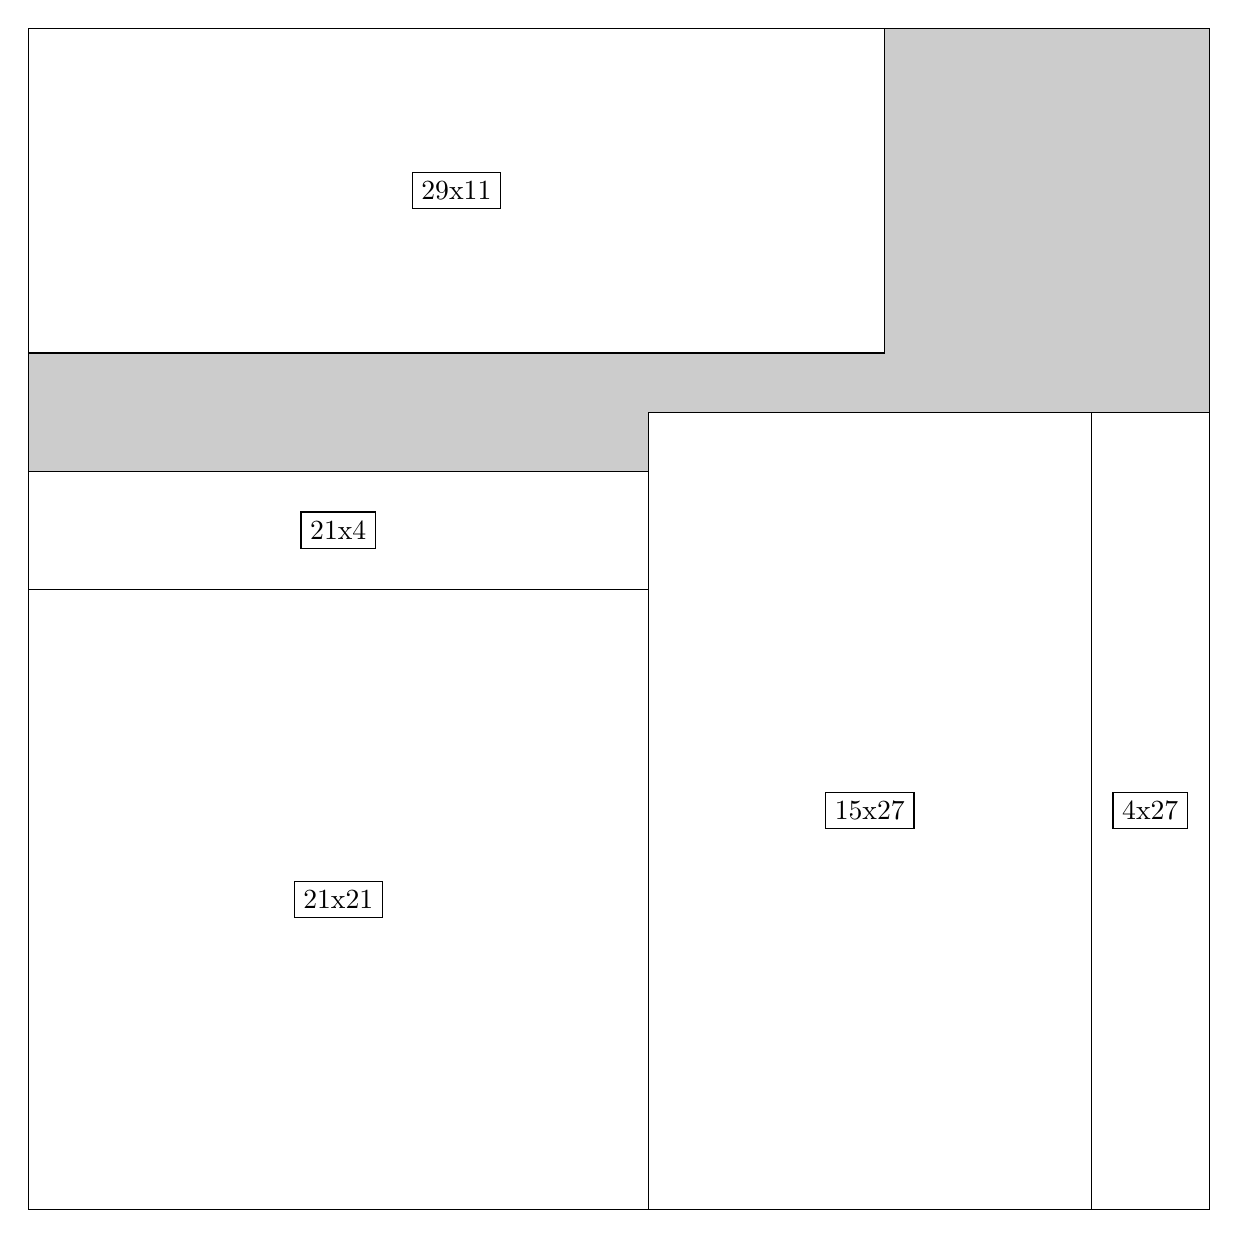
\begin{tikzpicture}[shorten >=1pt,scale=1.0,every node/.style={scale=1.0},->]
\tikzstyle{vertex}=[circle,fill=black!25,minimum size=14pt,inner sep=0pt]
\filldraw[fill=gray!40!white, draw=black] (0,0) rectangle (15.0,15.0);
\foreach \name/\x/\y/\w/\h in {21x21/0.0/0.0/7.875/7.875,15x27/7.875/0.0/5.625/10.125,29x11/0.0/10.875/10.875/4.125,4x27/13.5/0.0/1.5/10.125,21x4/0.0/7.875/7.875/1.5}
\filldraw[fill=white!40!white, draw=black] (\x,\y) rectangle node[draw] (\name) {\name} ++(\w,\h);
\end{tikzpicture}


w =21 , h =21 , x =0 , y =0 , v =441
\par
w =15 , h =27 , x =21 , y =0 , v =405
\par
w =29 , h =11 , x =0 , y =29 , v =319
\par
w =4 , h =27 , x =36 , y =0 , v =108
\par
w =21 , h =4 , x =0 , y =21 , v =84
\par
\newpage


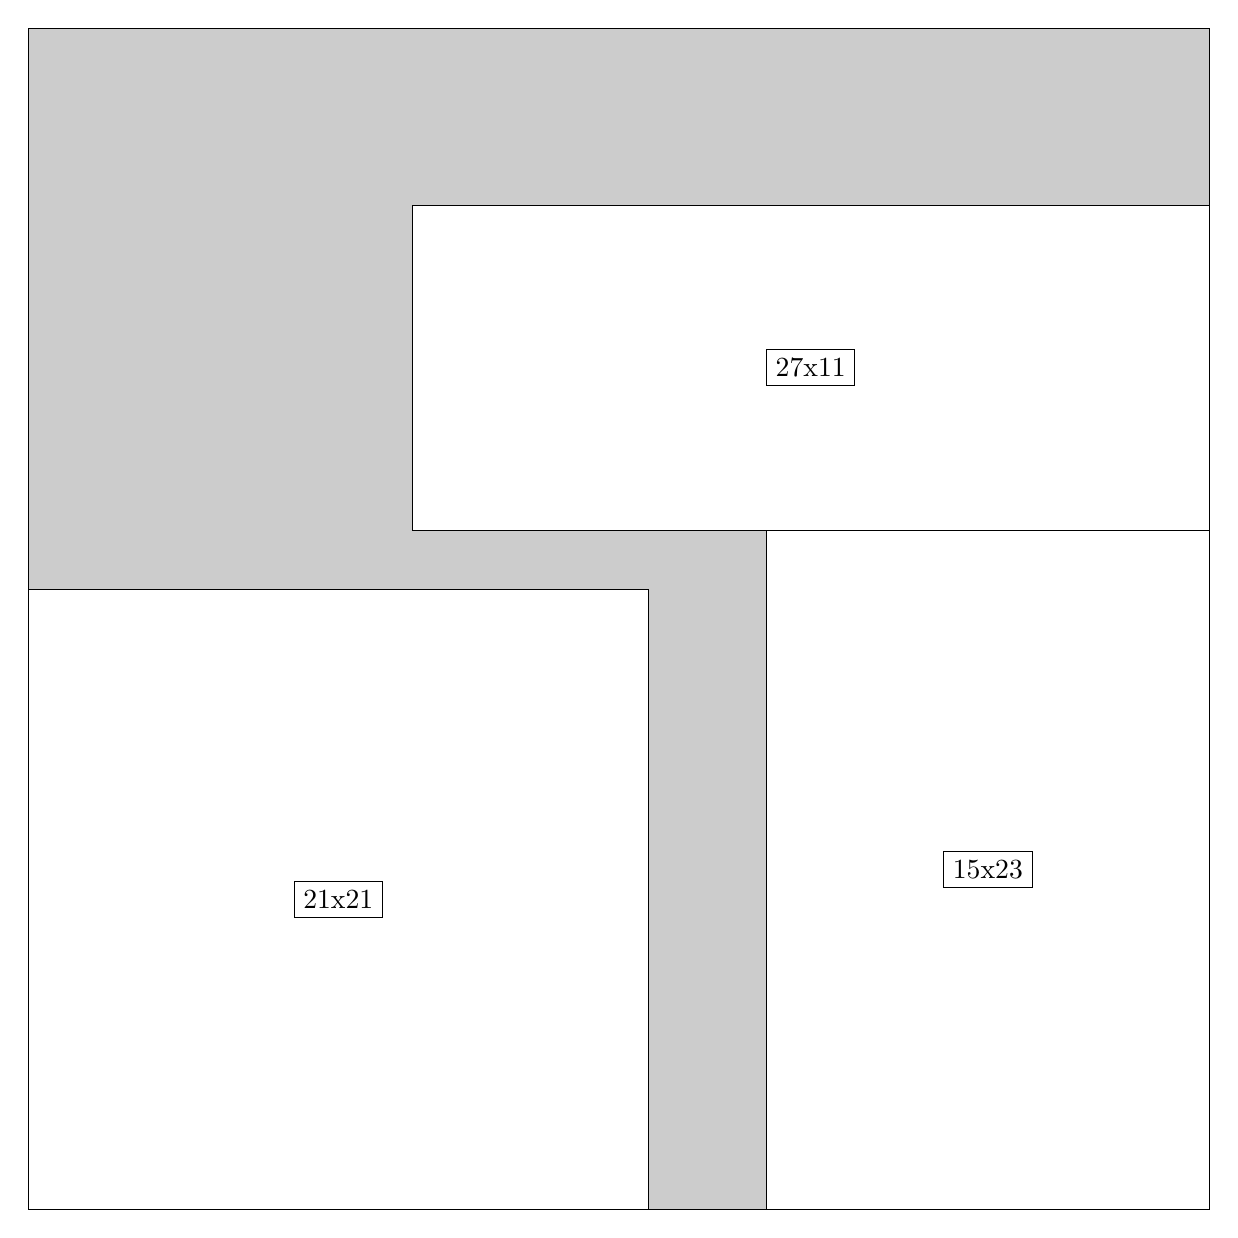
\begin{tikzpicture}[shorten >=1pt,scale=1.0,every node/.style={scale=1.0},->]
\tikzstyle{vertex}=[circle,fill=black!25,minimum size=14pt,inner sep=0pt]
\filldraw[fill=gray!40!white, draw=black] (0,0) rectangle (15.0,15.0);
\foreach \name/\x/\y/\w/\h in {21x21/0.0/0.0/7.875/7.875,15x23/9.375/0.0/5.625/8.625,27x11/4.875/8.625/10.125/4.125}
\filldraw[fill=white!40!white, draw=black] (\x,\y) rectangle node[draw] (\name) {\name} ++(\w,\h);
\end{tikzpicture}


w =21 , h =21 , x =0 , y =0 , v =441
\par
w =15 , h =23 , x =25 , y =0 , v =345
\par
w =27 , h =11 , x =13 , y =23 , v =297
\par
\newpage


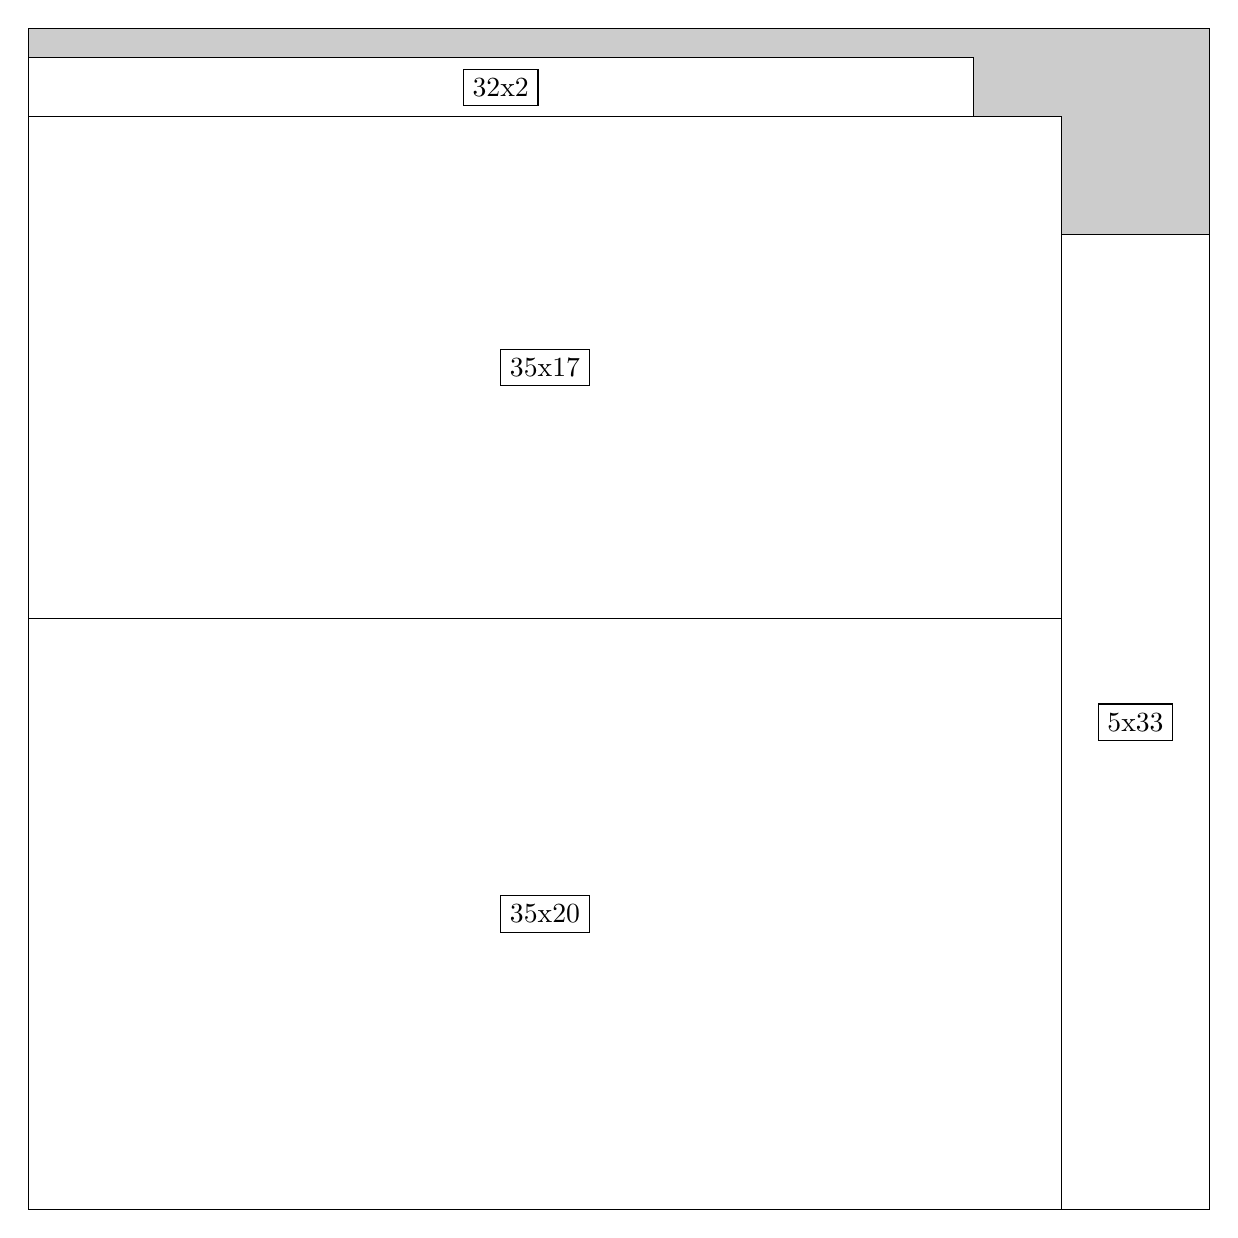
\begin{tikzpicture}[shorten >=1pt,scale=1.0,every node/.style={scale=1.0},->]
\tikzstyle{vertex}=[circle,fill=black!25,minimum size=14pt,inner sep=0pt]
\filldraw[fill=gray!40!white, draw=black] (0,0) rectangle (15.0,15.0);
\foreach \name/\x/\y/\w/\h in {35x20/0.0/0.0/13.125/7.5,35x17/0.0/7.5/13.125/6.375,5x33/13.125/0.0/1.875/12.375,32x2/0.0/13.875/12.0/0.75}
\filldraw[fill=white!40!white, draw=black] (\x,\y) rectangle node[draw] (\name) {\name} ++(\w,\h);
\end{tikzpicture}


w =35 , h =20 , x =0 , y =0 , v =700
\par
w =35 , h =17 , x =0 , y =20 , v =595
\par
w =5 , h =33 , x =35 , y =0 , v =165
\par
w =32 , h =2 , x =0 , y =37 , v =64
\par
\newpage


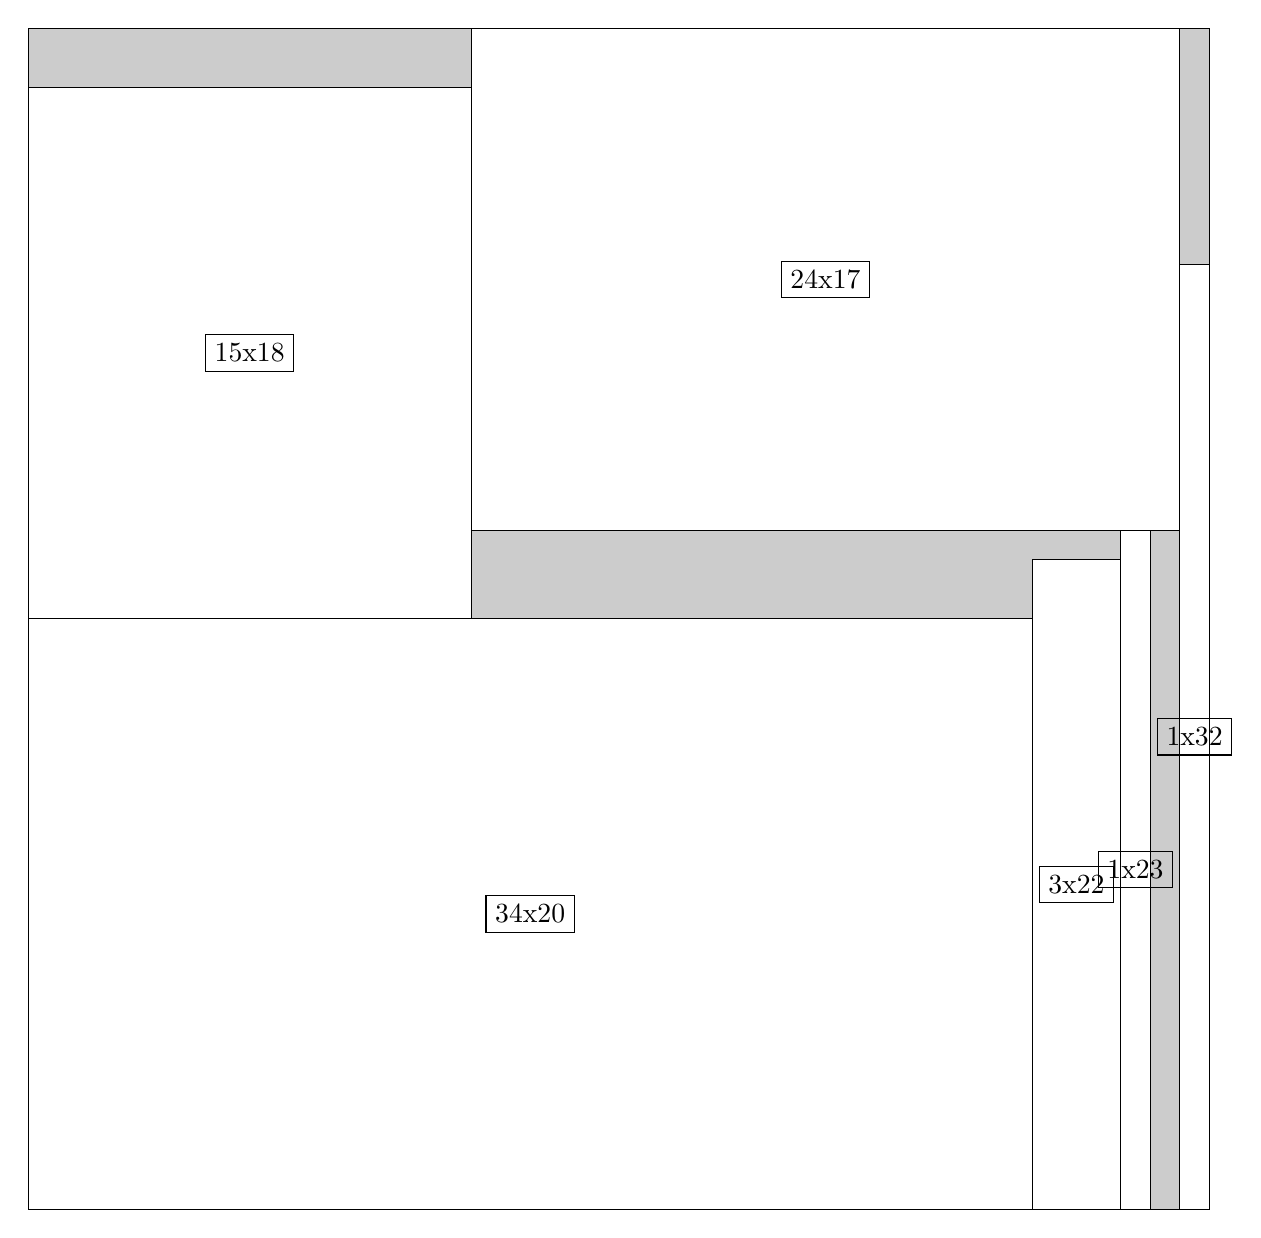
\begin{tikzpicture}[shorten >=1pt,scale=1.0,every node/.style={scale=1.0},->]
\tikzstyle{vertex}=[circle,fill=black!25,minimum size=14pt,inner sep=0pt]
\filldraw[fill=gray!40!white, draw=black] (0,0) rectangle (15.0,15.0);
\foreach \name/\x/\y/\w/\h in {34x20/0.0/0.0/12.75/7.5,24x17/5.625/8.625/9.0/6.375,15x18/0.0/7.5/5.625/6.75,3x22/12.75/0.0/1.125/8.25,1x32/14.625/0.0/0.375/12.0,1x23/13.875/0.0/0.375/8.625}
\filldraw[fill=white!40!white, draw=black] (\x,\y) rectangle node[draw] (\name) {\name} ++(\w,\h);
\end{tikzpicture}


w =34 , h =20 , x =0 , y =0 , v =680
\par
w =24 , h =17 , x =15 , y =23 , v =408
\par
w =15 , h =18 , x =0 , y =20 , v =270
\par
w =3 , h =22 , x =34 , y =0 , v =66
\par
w =1 , h =32 , x =39 , y =0 , v =32
\par
w =1 , h =23 , x =37 , y =0 , v =23
\par
\newpage


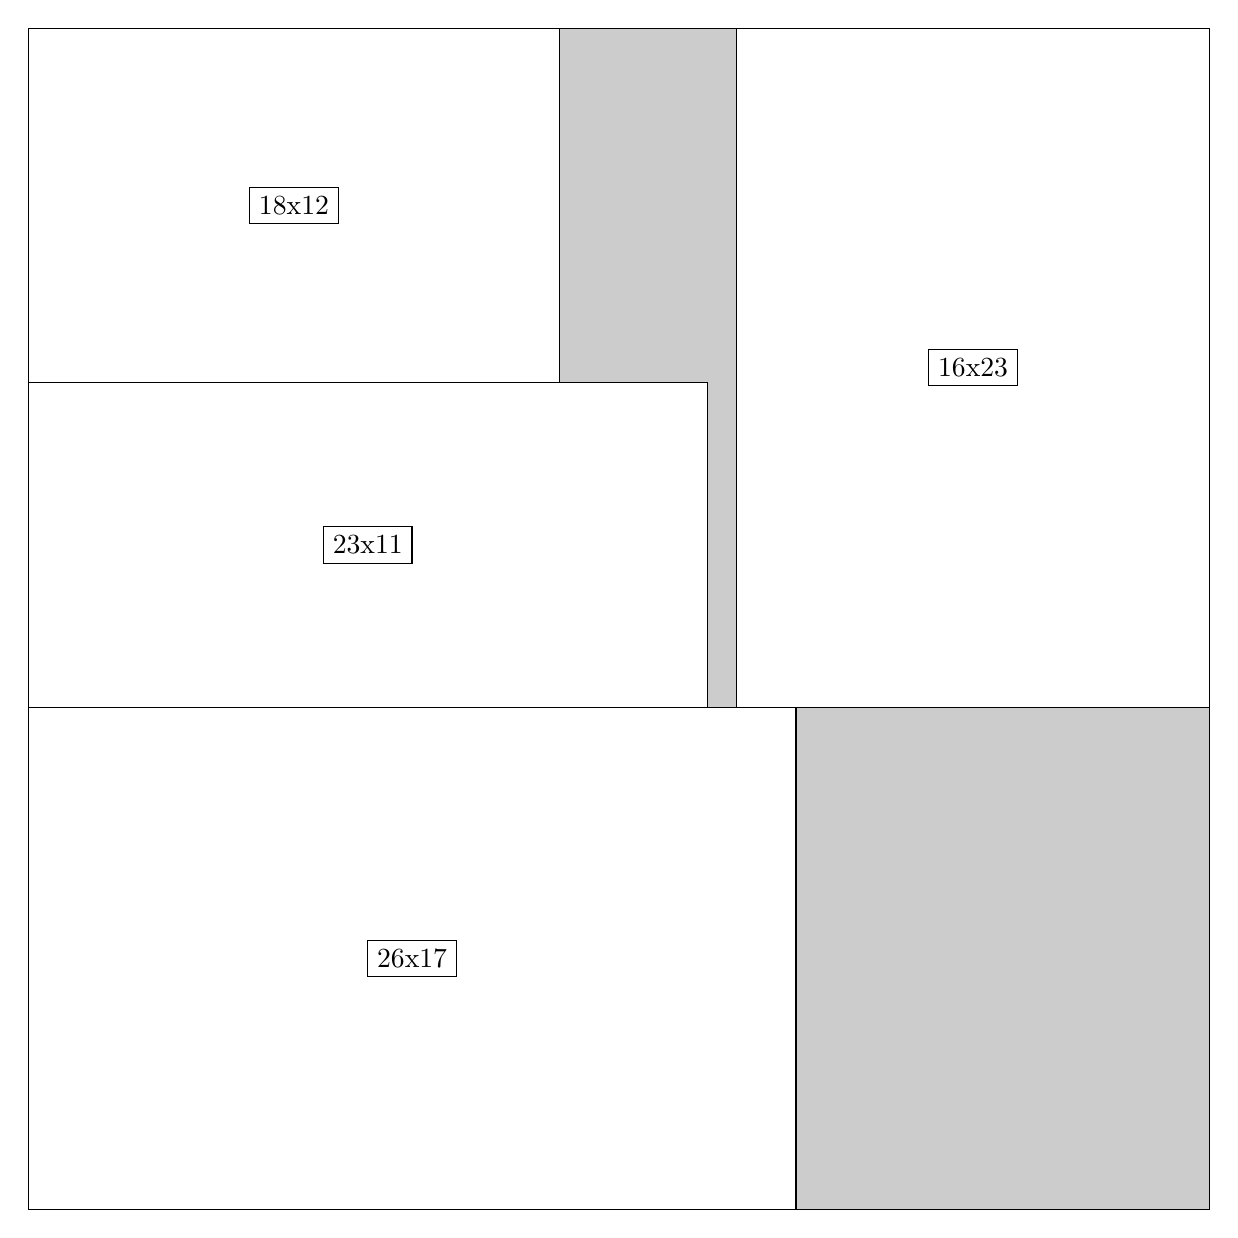
\begin{tikzpicture}[shorten >=1pt,scale=1.0,every node/.style={scale=1.0},->]
\tikzstyle{vertex}=[circle,fill=black!25,minimum size=14pt,inner sep=0pt]
\filldraw[fill=gray!40!white, draw=black] (0,0) rectangle (15.0,15.0);
\foreach \name/\x/\y/\w/\h in {26x17/0.0/0.0/9.75/6.375,23x11/0.0/6.375/8.625/4.125,16x23/9.0/6.375/6.0/8.625,18x12/0.0/10.5/6.75/4.5}
\filldraw[fill=white!40!white, draw=black] (\x,\y) rectangle node[draw] (\name) {\name} ++(\w,\h);
\end{tikzpicture}


w =26 , h =17 , x =0 , y =0 , v =442
\par
w =23 , h =11 , x =0 , y =17 , v =253
\par
w =16 , h =23 , x =24 , y =17 , v =368
\par
w =18 , h =12 , x =0 , y =28 , v =216
\par
\newpage


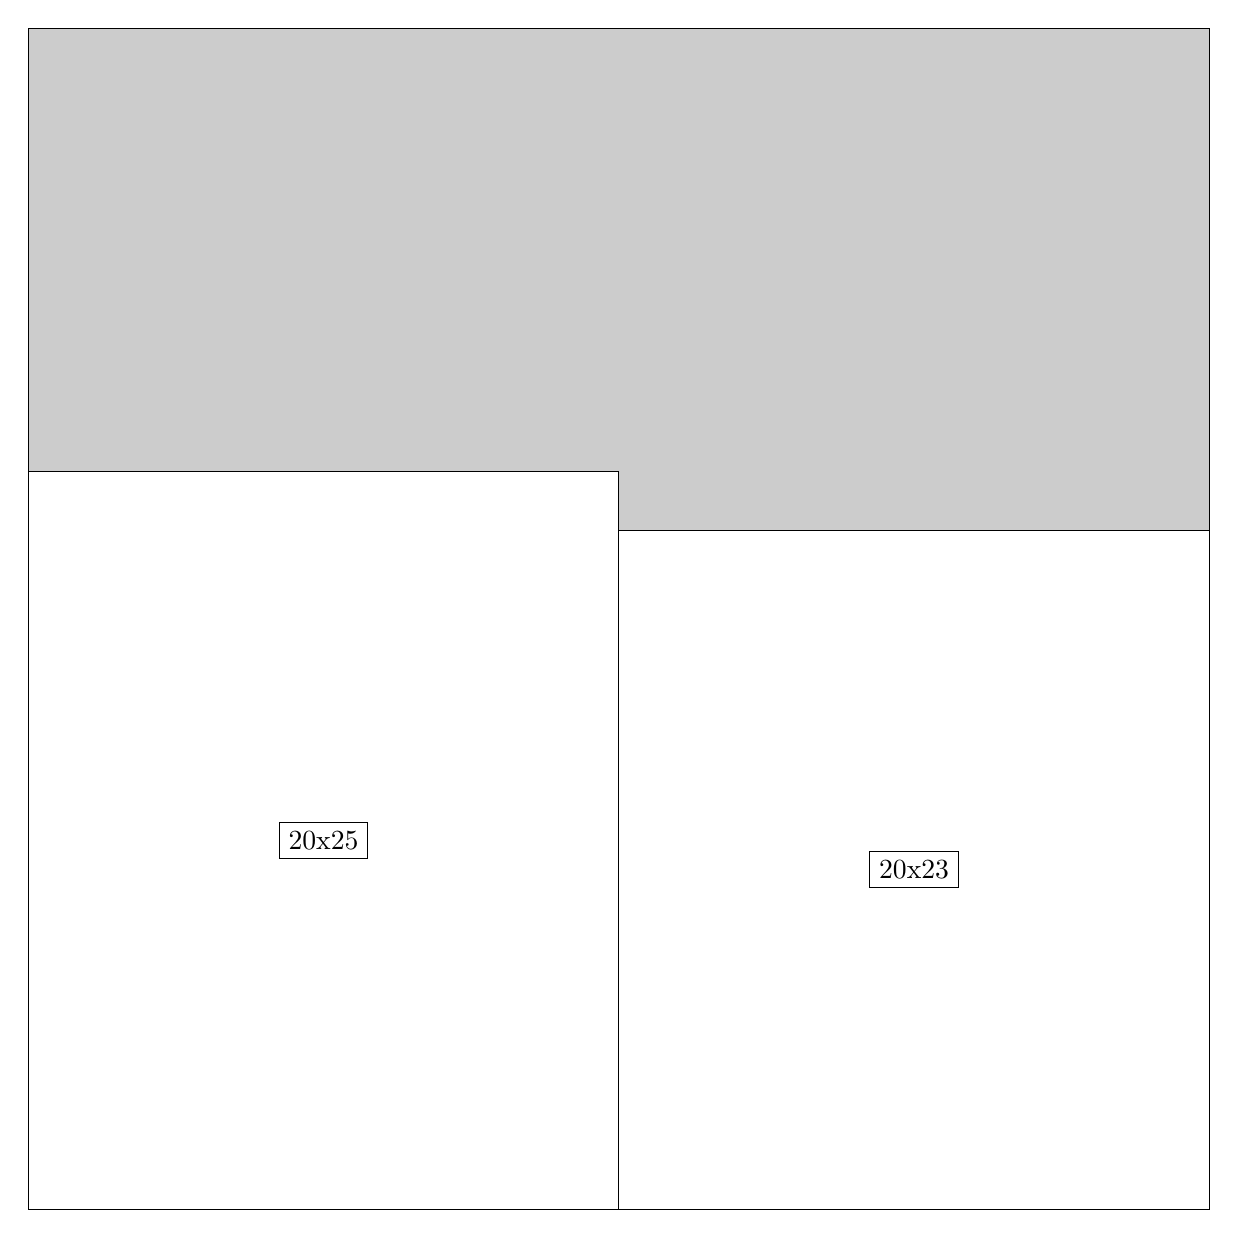
\begin{tikzpicture}[shorten >=1pt,scale=1.0,every node/.style={scale=1.0},->]
\tikzstyle{vertex}=[circle,fill=black!25,minimum size=14pt,inner sep=0pt]
\filldraw[fill=gray!40!white, draw=black] (0,0) rectangle (15.0,15.0);
\foreach \name/\x/\y/\w/\h in {20x25/0.0/0.0/7.5/9.375,20x23/7.5/0.0/7.5/8.625}
\filldraw[fill=white!40!white, draw=black] (\x,\y) rectangle node[draw] (\name) {\name} ++(\w,\h);
\end{tikzpicture}


w =20 , h =25 , x =0 , y =0 , v =500
\par
w =20 , h =23 , x =20 , y =0 , v =460
\par
\newpage


\end{document}